\def\thoigian{90}%--Thời gian
\de{ĐỀ THI THỬ MÔN TOÁN NĂM HỌC 2025-2026}{THPT LÊ THÁNH TÔNG - TPHCM}
\Opensolutionfile{ans}[ans/ans-HK2-LTT-HCM-25-26] 

\begin{center}
	\textbf{PHẦN 1 - TRẮC NGHIỆM}
\end{center}
%Câu 1
\begin{ex}%[Đề thi thử môn Toán THPT Lê Thánh Tông - TPHCM năm học 2025-2026]%[Phạm Văn Long - Nguyễn Thanh Phong]%[1D2N2-4]
	Cấp số cộng $\left(u_n \right)$ có $u_1=-1$ và $u_2=3$. Số hạng $u_5$ của cấp số cộng bằng
	\choice
	{\True $15$}
	{$5$}
	{$9$}
	{$13$}
	\loigiai{Ta có $u_5=u_1+4d=-1+4\cdot 4=15$.
	}
\end{ex}
%%%==============HetCau_EX1==============%%%

%%%==============Cau_EX2==============%%%
 \begin{ex}%[Đề thi thử môn Toán THPT Lê Thánh Tông - TPHCM năm học 2025-2026]%[Phạm Văn Long - Nguyễn Thanh Phong]%[1D6H4-3]
	Tập nghiệm của bất phương trình $\log_3 (x+1)\le 2$ là
	\choice
	{$(1;9)$}
	{$(-1;7]$}
	{$(-\infty;9]$}
	{\True $(-1;8]$}
	\loigiai{
		Điều kiện là $x+1> 0\Leftrightarrow x >-1$.\\		
		$\log_3 (x+1)\le 2\Leftrightarrow x+1\le 9\Leftrightarrow x\le 8$.\\
		Kết hợp với điều kiện, bất phương trình có tập nghiệm là $S=(-1;8]$.
	}
\end{ex}
%%%==============HetCau_EX2==============%%%

%%%==============Cau_EX3==============%%%
\begin{ex}%[Đề thi thử môn Toán THPT Lê Thánh Tông - TPHCM năm học 2025-2026]%[Phạm Văn Long - Nguyễn Thanh Phong]%[2D1N1-2]
	\immini{Cho hàm số có đồ thị $y=f(x)$ như hình vẽ bên dưới. Hàm số đã cho nghịch biến trên khoảng nào sau đây?
	\choice
	{$(-1;\; 1)$}
	{$(-\infty;\; 1)$}
	{\True $(-\infty;\;-1)$}
	{$(-1;+\infty)$}}
	{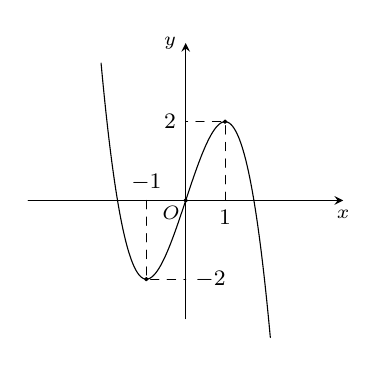
\begin{tikzpicture}[scale=0.5, font=\footnotesize,line join=round, line cap=round, >=stealth]
			\draw[->] (-4,0) -- (4,0) node[below] {\scriptsize $x$};
			\draw[->] (0,-3) -- (0,4) node[left] {\scriptsize $y$};
			\draw (0.1,0.1)node[below left]{\scriptsize $O$};
			\draw[thin,samples=150,smooth,domain=-2.15:2.15] plot(\x,{-1*((\x)^3)-0*((\x)^2)+3*(\x)+0});		
			\draw[dashed] (-1,0)node[above]{$-1$} -- (-1,-2)--(0,-2)node[right]{$-2$}
			(1,0)node[below]{$1$} -- (1,2)--(0,2)node[left]{$2$};
			\draw[fill=black]  (-1,-2) circle (1.2pt) (1,2) circle (1.2pt) (0,0) circle (1.2pt);
	\end{tikzpicture}}
	\loigiai{
		Từ giả thiết ta có hàm số nghịch biến trên $(-\infty;-1)$. 
	}
\end{ex}
%%%==============HetCau_EX3==============%%%

%%%==============Cau_EX4==============%%%
\begin{ex}%[Đề thi thử môn Toán THPT Lê Thánh Tông - TPHCM năm học 2025-2026]%[Phạm Văn Long - Nguyễn Thanh Phong]%[2D1H2-1]
	Cho hàm số $y=f(x)$ liên tục trên $\mathbb{R}$ và có đạo hàm là $f'(x)=x^2\left(x^2-5x+4\right)$, $\forall x\in \mathbb{R}$. Hàm số $f(x)$ có bao nhiêu điểm cực tiểu?
	\choice
	{$0$}
	{$2$}
	{\True $1$}
	{$3$}
	\loigiai{
		Ta có $f'(x)=x^2\left(x^2-5x+4\right)=0\Leftrightarrow \hoac{&x=0 \,\text{(nghiệm kép)}\\&x=4\\&x=1.}$\\
		Bảng xét dấu
			\begin{center}
			
\begin{tikzpicture}
				\tkzTabInit[lgt=1.2,espcl=2.5,deltacl=0.6]
				{$x$ /0.6,$f'(x)$ /0.6}
				{$-\infty$,$1$,$4$,$+\infty$}
				\tkzTabLine{,+,$0$,-,$0$,+,}
			\end{tikzpicture}
		\end{center}
		Vậy hàm số có $1$ điểm cực tiểu.
	}
\end{ex}
%%%==============HetCau_EX4==============%%%

%%%==============Cau_EX5==============%%%
\begin{ex}%[Đề thi thử môn Toán THPT Lê Thánh Tông - TPHCM năm học 2025-2026]%[Phạm Văn Long - Nguyễn Thanh Phong]%[2D1H3-1]
	Giá trị nhỏ nhất của hàm số $y=\sqrt{16-x^2}$ trên đoạn $[-2;2]$ bằng
	\choice
	{$4$}
	{\True $2\sqrt{3}$}
	{$2\sqrt{5}$}
	{$0$}
	\loigiai{
		Ta có $y'=\dfrac{-2x}{2\sqrt{16-x^2}}=\dfrac{-x}{\sqrt{16-x^2}}$.\\
		$y'=0\Rightarrow x=0\in [-2;2]$.\\
		Khi đó $y(-2)=y(2)=\sqrt{16-4}=2\sqrt{3}$; $y(0)=\sqrt{16}=4$.\\		
		Suy ra ${\mathop{\min}\limits_{\left[-2;2\right]}} y=y\left(-2\right)=y(2)=2\sqrt{3}$.
	}
\end{ex}
%%%==============HetCau_EX5==============%%%

%%%==============Cau_EX6==============%%%
\begin{ex}%[Đề thi thử môn Toán THPT Lê Thánh Tông - TPHCM năm học 2025-2026]%[Phạm Văn Long - Nguyễn Thanh Phong]%[2H2H1-3]
	Trong không gian, cho hai vectơ $\overrightarrow{u}$ và $\overrightarrow{v}$ thỏa mãn $\left|\overrightarrow{u}\right|=5$, $\left|\overrightarrow{v}\right|=8$ và $\left(\overrightarrow{u},\overrightarrow{v}\right)=120^\circ$. Khẳng định nào dưới đây là đúng?
	\choice
	{$\overrightarrow{u}\cdot \overrightarrow{v}=20$}
	{$\overrightarrow{u}\cdot \overrightarrow{v}=-20\sqrt{3}$}
	{\True $\overrightarrow{u}\cdot \overrightarrow{v}=-20$}
	{$\overrightarrow{u}\cdot \overrightarrow{v}=40$}
	\loigiai{
		Ta có $\vec{u}\cdot \vec{v}=\left|\vec{u}\right|\cdot \left|\vec{v}\right|\cdot \cos \left(\vec{u},\vec{v}\right)=5\cdot 8\cdot \cos 120^{\circ}=-20$.
	}
\end{ex}
%%%==============HetCau_EX6==============%%%

%%%==============Cau_EX7==============%%%
\begin{ex}%[Đề thi thử môn Toán THPT Lê Thánh Tông - TPHCM năm học 2025-2026]%[Phạm Văn Long - Nguyễn Thanh Phong]%[2H2V1-2]
	Cho hình chóp $S.ABCD$, có đáy $ABCD$ là hình thoi, $SA=AB=2$, $\widehat{ABC}=60^{\circ}$, $SA$ vuông góc với mặt đáy. Gọi $H$ là trung điểm của $SA$. Tính $D=\left|2\overrightarrow{SH}+\overrightarrow{AD}-2\overrightarrow{BH}\right|$.
	\choice
	{\True $2\sqrt{7}$}
	{$2\sqrt{2}$}
	{$\sqrt{5}$}
	{$4$}
	\loigiai{
		Ta có $ABCD$ là hình thoi $\Rightarrow BA=BC$ $\Rightarrow \triangle ABC$ cân tại $B$.\\
		Lại có $\widehat{ABC}=60^{\circ}$ $\Rightarrow \triangle ABC$ cân là tam giác đều $\Rightarrow BA=BC=AC=2$.\\
		Suy ra $\triangle SAB=\triangle SAC$ (c-g-c) $\Rightarrow SB=SC$.\\
		Do đó $\triangle SBC$ cân tại $S$.\\
		Gọi $I$ là trung điểm của $BC$ thì ta có\\
		$SI\perp BC\Rightarrow SI^2=SB^2-BI^2=SA^2+AB^2-\left(\dfrac{1}{2} BC\right)^2=2^2+2^2-1^2=7$.\\		
		$2\overrightarrow{SH}+\overrightarrow{AD}-2\overrightarrow{BH}=2\left(\overrightarrow{SH}+\overrightarrow{HB}\right)+\overrightarrow{BC}=\overrightarrow{SB}+\overrightarrow{SB}+\overrightarrow{BC}=\overrightarrow{SB}+\overrightarrow{SC}=2\overrightarrow{SI}$.\\
		Suy ra $D^2=\left(\left|2\overrightarrow{SI}\right|\right)^2=2^2\cdot 7\Rightarrow D=2\sqrt{7}$.
	}
\end{ex}
%%%==============HetCau_EX7==============%%%

%%%==============Cau_EX8==============%%%
\begin{ex}%[Đề thi thử môn Toán THPT Lê Thánh Tông - TPHCM năm học 2025-2026]%[Phạm Văn Long - Nguyễn Thanh Phong]%[2H2H2-3]
	Trong không gian $Oxyz$, tam giác $ABC$ có $\overrightarrow{AB}=(-2;-5;0)$, $\overrightarrow{AC}=(2;-2;0)$. Độ dài đoạn thẳng $BC$ bằng
	\choice
	{$1$}
	{\True $5$}
	{$3$}
	{$\sqrt{10}$}
	\loigiai{
		Ta có $\overrightarrow{BC}=\overrightarrow{AC}-\overrightarrow{AB}=\left(4;3;0\right)$ $\Rightarrow BC=\sqrt{4^2+3^2}=5$.
	}
\end{ex}
%%%==============HetCau_EX8==============%%%

%%%==============Cau_EX9==============%%%
\begin{ex}%[Đề thi thử môn Toán THPT Lê Thánh Tông - TPHCM năm học 2025-2026]%[Phạm Văn Long - Nguyễn Thanh Phong]%[1D7V2-1]
	Cho $a$, $b$ là hai số thực dương khác $1$ thỏa mãn đồ thị hàm số $y=f(x)=\log_a x+\log_b x$ luôn đi qua điểm $M(\mathrm{e};20)$. Tính đạo hàm của hàm số tại điểm $x=5$.
	\choice
	{$15$}
	{$\dfrac{1}{15}$}
	{\True $4$}
	{$\dfrac{e}{4}$}
	\loigiai{
		Tập xác định $\mathscr{D}=(0;+\infty)$.\\
		Do đồ thị hàm số luôn đi qua điểm $M(\mathrm{e};20)$ nên 
		$$20=f(\mathrm{e})=\log_a \mathrm{e}+\log_b \mathrm{e}=\dfrac{1}{\ln a}+\dfrac{1}{\ln b}.$$
		Ta có $y'=f'(x)=\dfrac{1}{x\cdot \ln a}+\dfrac{1}{x\cdot \ln b}$.\\		
		Khi đó $y'(5)=f'(5)=\dfrac{1}{5\ln a}+\dfrac{1}{5\ln b}=\dfrac{1}{5}\cdot \left(\dfrac{1}{\ln a}+\dfrac{1}{\ln b} \right)=\dfrac{1}{5}\cdot 20=4.$
	}
\end{ex}
%%%==============HetCau_EX9==============%%%

%%%==============Cau_EX10==============%%%
\begin{ex}%[Đề thi thử môn Toán THPT Lê Thánh Tông - TPHCM năm học 2025-2026]%[Phạm Văn Long - Nguyễn Thanh Phong]%[1D7H2-3]
	Tiếp tuyến của đồ thị hàm số $y=\dfrac{2x+3}{x-2}$ tại điểm có hoành độ bằng $3$ có phương trình là
	\choice
	{$y=7x+13$}
	{\True $y=30-7x$}
	{$y=3x+9$}
	{$y=-\dfrac{4}{3} x-2$}
	\loigiai{
		Tập xác định $\mathscr{D}=\mathbb{R}\setminus \{2\}$.\\
		Ta có $y'=\dfrac{-7}{\left(x-2\right)^2}$ suy ra $y'(3)=\dfrac{-7}{\left(3-2\right)^2}=-7$, $y(3)=\dfrac{2\cdot 3+3}{3-2}=9$.\\
		Tiếp tuyến của đồ thị hàm số $y=\dfrac{2x+3}{x-2}$ tại điểm có hoành độ bằng $3$ có phương trình là $$y=-7\left(x-3\right)+9\Leftrightarrow y=-7x+30.$$
	}
\end{ex}
%%%==============HetCau_EX10==============%%%

%%%==============Cau_EX11==============%%%
\begin{ex}%[Đề thi thử môn Toán THPT Lê Thánh Tông - TPHCM năm học 2025-2026]%[Phạm Văn Long - Nguyễn Thanh Phong]%[2D1H1-1]
	Cho hàm số $y=f(x)=\dfrac{1}{2} x^2+x-6\ln x+2025$ nghịch biến trên khoảng nào sau đây?
	\choice
	{$(-3;2)$}
	{$(2;+\infty)$}
	{$(0;3)$}
	{\True $(0;1)$}
	\loigiai{
		Tập xác định $\mathscr{D}=(0;+\infty)$.\\
		Ta có $f'(x)=x+1-\dfrac{6}{x}=\dfrac{x^2+x-6}{x}$.\\		
		Khi đó $f'(x)=0\Rightarrow x^2+x-6=0\Rightarrow \hoac{&x=-3\\&x=2.}$\\
		Bảng biến thiên
		\begin{center}
			
\begin{tikzpicture}
				\tkzTabInit[lgt=1.2,espcl=2.5,deltacl=0.6]
				{$x$ /0.6,$f'(x)$ /0.6}
				{$0$,$2$,$+\infty$}
				\tkzTabLine{,-,$0$,+,}
			\end{tikzpicture}
		\end{center}
		Hàm số nghịch biến trên $(0;2)$. Do đó hàm số nghịch biến trên $(0;1)$.
	}
\end{ex}
%%%==============HetCau_EX11==============%%%

%%%==============Cau_EX12==============%%%
\begin{ex}%[Đề thi thử môn Toán THPT Lê Thánh Tông - TPHCM năm học 2025-2026]%[Phạm Văn Long - Nguyễn Thanh Phong]%[2D1H3-6]
	Một cửa hàng buôn giày nhập một đôi với giá là $40$ đôla. Cửa hàng ước tính rằng nếu đôi giày được bán với giá $x$ đôla thì mỗi tháng khách hàng sẽ mua $\left(120-x\right)$ đôi. Hỏi cửa hàng bán một đôi giày giá bao nhiêu thì thu được nhiều lãi nhất?
	\choice
	{\True $80$ USD}
	{$160$ USD}
	{$40$ USD}
	{$240$ USD}
	\loigiai{
		Lãi mỗi đôi giày là $x-40$ đôla $(40\le x\le 120)$.\\		
		Tiền lãi khi bán được $\left(120-x\right)$ đôi giày là $$f(x)=\left(x-40\right)\cdot \left(120-x\right)=-x^2+160x-4800.$$		
		Ta có $f'(x)=-2x+160$.\\
		$f'(x)=0\Leftrightarrow-2x+160=0\Leftrightarrow x=80$.\\
		Bảng biến thiên
			\begin{center}
			
\begin{tikzpicture}
				\tkzTabInit[lgt=1.2,espcl=2.5,deltacl=0.6]
				{$x$ /0.6,$f'(x)$ /0.6,$f(x)$ /2}
				{$40$,$80$,$120$}
				\tkzTabLine{,+,$0$,-,}
				\tkzTabVar{ -/$ $,+/$1600$,-/$ $}
			\end{tikzpicture}
		\end{center}
		Vậy cửa hàng cần bán giày với giá $80$ USD một đôi thì thu được nhiều lãi nhất.
	}
\end{ex}
%%%==============HetCau_EX12==============%%%
\begin{center}
	\textbf{PHẦN 2 - Câu trắc nghiệm đúng sai. Trong mỗi ý a,b,c,d ở mỗi câu, thí sinh chọn đúng hoặc sai}
\end{center}
\setcounter{ex}{0} 
%==================Câu 1========================
\begin{ex}%[2D1V3-6]%[Dự án đề kiểm tra Toán khối 11 HKI NH2025-2026-Đợt 4]%[Tên Giáo Viên]
	Lợi nhuận thu được $P$ (nghìn USD) của một công ty khi dùng số tiền $x$ (nghìn USD) chi cho quảng cáo được cho bởi công thức $P(x) = -\dfrac{1}{10}x^3 + 6x^2 + 400$ với $x \ge 0$.
	\choiceTF
	{Lợi nhuận của công ty tăng khi số tiền chi cho quảng cáo tăng}
	{\True Có hai phương án giúp công ty có thể thu được lợi nhuận bằng $800$ nghìn USD}
	{Hàm số $P = P(x)$ có hai điểm cực trị}
	{\True Lợi nhuận tối đa mà công ty thu được bằng $3{,}6$ triệu USD}
	\loigiai{
		Ta có $P'(x) = -\dfrac{3}{10}x^2 + 12x=0 \Leftrightarrow \hoac{&x=0\\&x=40.}$\\
		Ta có bảng biến thiên:
		\begin{center}
			
\begin{tikzpicture}[scale=1,font=\footnotesize,line join=round,line cap=round,>=stealth]
				\tkzTabInit
				[lgt=1.5,espcl=4] 
				{$x$/0.6, $P'(x)$/0.7, $P(x)$/2} 
				{$0$, $40$, $+\infty$}
				\tkzTabLine{,+,0,-,} 
				\tkzTabVar{-/ $400$, +/ $3600$ , -/ $-\infty$}
				% \draw[color=red!80!black] (2.5,-2.5)--(9.5,-2.5)node[above]{$y=800$};
			\end{tikzpicture}
		\end{center}
		\begin{itemchoice}
			\itemch Khi $x > 40$ thì lợi nhuận giảm.
			\itemch Xét phương trình $P(x)=800 \Leftrightarrow -\dfrac{1}{10}x^3 + 6x^2 + 400=800 \Leftrightarrow \hoac{&x\approx 58{,}84\\&x \approx 8{,}84.}$\\
			Vậy có $2$ phương án giúp công ty có thể thu được lợi nhuận bằng $800$ nghìn USD.
			\itemch Dựa vào bảng biến thiên ở trên, ta thấy hàm số $P=P(x)$ có $1$ điểm cực trị.
			\itemch Dựa vào bảng biến thiên, $\max\limits_{[0;+\infty)} P(x) = P(40) = 3600$ (nghìn USD) $= 3{,}6$ (triệu USD).
		\end{itemchoice}
	}
\end{ex}

\begin{ex}%[2D1V2-1]%[Dự án đề kiểm tra ...]
	Cho hàm số $y = f(x) = \dfrac{x^2+2x+4}{x+2}$.
	\choiceTF
	{\True Hàm số đã cho đồng biến trên khoảng $(0;+\infty)$}
	{Gọi $A, B$ là các điểm cực đại, cực tiểu của đồ thị hàm số. Diện tích của tam giác $OAB$ bằng $8$, trong đó $O$ là gốc tọa độ}
	{\True Đường thẳng đi qua hai điểm cực trị của đồ thị hàm số là $y = 2x +2$}
	{Tổng giá trị lớn nhất và giá trị nhỏ nhất của hàm số trên đoạn $[-3;3]$ bằng $-3{,}2$}
	\loigiai{
		Tập xác định: $\mathscr{D} = \mathbb{R} \setminus \{-2\}$. \\
		Ta có $y' = \dfrac{x^2+4x}{(x+2)^2} = 0 \Leftrightarrow \hoac{&x = 0\\&x = -4.}$\\
		Ta có bảng biến thiên:
		\begin{center}
			
\begin{tikzpicture}
				\tkzTab
				[lgt=2,espcl=2]
				{$x$/0.7, $f'(x)$/0.7, $f(x)$/2} 
				{$-\infty$, $-4$, $-2$, $0$, $+\infty$} 
				{,+,0,-,d,-,0,+,}
				{-/ $-\infty$, +/ $-6$, -D+/ $-\infty$ / $+\infty$, -/ $2$, +/ $+\infty$} 
			\end{tikzpicture}
		\end{center}
		\begin{itemchoice}
			\itemch Dựa vào bảng biến thiên ta thấy hàm số đồng biến trên khoảng $(0;+\infty)$.
			\itemch Các điểm cực trị là $A(-4;-6)$ và $B(0;2)$. \\
			Vì $B \in Oy$ nên $S_{\triangle OAB} = \dfrac{1}{2} \cdot OB \cdot \mathrm{d}(A,Oy) = \dfrac{1}{2} \cdot 2 \cdot 4 = 4 \ne 8$.
			\itemch Phương trình đường thẳng đi qua $2$ điểm $A(-4;-6)$ và $B(0;2)$ là $d\colon \dfrac{x}{4}=\dfrac{y-2}{8}$. \\
			Suy ra  $d\colon y=2x+2$. 
			\itemch Hàm số không xác định tại $x = -2 \in [-3;3]$ nên không tồn tại $\max$, $\min$ trên đoạn này.
		\end{itemchoice}
	}
\end{ex}

\begin{ex}%[2D1V3-6]%[Dự án đề kiểm tra ...]
	Bạn An làm đèn lồng bằng cách dùng một sợi dây đồng dài $28$ dm cắt thành ba đoạn để uốn làm khung đèn. Đoạn thứ nhất uốn thành hình vuông $ABCD$ có cạnh bằng $x$ (dm) để làm đáy, hai đoạn còn lại có độ dài bằng nhau uốn thành các đường gấp khúc $ASC$ và $BSD$. Khung đèn sau khi hoàn thiện có hình dạng là một hình chóp tứ giác đều $S.ABCD$ và bề mặt ngoài của đèn được dán giấy màu để trang trí, không dán mặt đáy (\textit{xem các mối nối, dán là không đáng kể}).
	\choiceTF
	{\True Độ dài cạnh bên của khung đèn bằng $(7 - x)$ dm với $0 < x < 7$}
	{\True Khi $x = 4$ thì độ dài đường cao của khung đèn là $1$ dm}
	{Khi các cạnh bằng nhau thì diện tích giấy màu cần dùng là $14\sqrt{3}$ dm$^2$}
	{\True Thể tích phần không gian của đèn lồng lớn nhất khi $x \approx 3{,}25$ dm}
	\loigiai{
		\begin{center}
			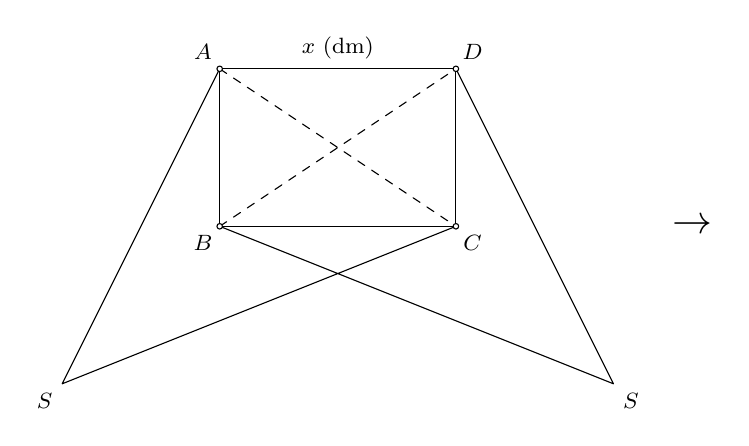
\begin{tikzpicture}[line join=round, line cap=round, font=\footnotesize]
				\path (0,0) coordinate (A)
				(0,-2) coordinate (B)
				(3,-2) coordinate (C)
				(3,0) coordinate (D)
				(-2,-4) coordinate (S_1)
				(5,-4) coordinate (S_2);
				\draw (A)--(B)--(C)--(D)--(A)node[above, midway]{$x$ (dm)}; 
				\draw[dashed] (A)--(C) (B)--(D);
				\draw (A)--(S_1)node[below left]{$S$}--(C) (D)--(S_2)node[below right]{$S$}--(B);
				\foreach \d/\g in {A/135, B/-135, C/-45, D/45}
				\draw[fill=white] (\d) circle(1pt) node[shift={(\g:.3)}]{$\d$};
				\node at (6, -2) {\Large $\rightarrow$};
			\end{tikzpicture}
			\begin{tikzpicture}[line cap=round,line join=round,font=\footnotesize]
				\path (0:0) coordinate(B) 
				(45:2.3) coordinate(A) 
				(0:4) coordinate(C) 
				($(A)+(C)-(B)$) coordinate(D) 
				(60:5.5) coordinate(S) 
				($(A)!.5!(C)$) coordinate(O);
				\draw (S)--(B)--(C)--(D)--cycle (S)--(C);
				\draw[dashed] (S)--(A)--(B)--(D)--(A)--(C) (S)--(O);
				\foreach \d/\g in {A/180, B/-135, C/-45, D/0, S/90, O/-95}
				\draw[fill=white] (\d) circle(1pt) node[shift={(\g:.3)}]{$\d$};
				\coordinate (O_S) at ($(O)!0.2cm!(S)$);
				\coordinate (O_D) at ($(O)!0.2cm!(D)$);
				\coordinate (O_A) at ($(O)!0.2cm!(A)$);
				\draw (O_S) -- ($(O_S)+(O_D)-(O)$) -- (O_D);
				\draw (O_S) -- ($(O_S)+(O_A)-(O)$) -- (O_A);
			\end{tikzpicture}
		\end{center}
		Khối chóp tứ giác đều có $4$ cạnh đáy bằng $x$ và $4$ cạnh bên bằng $l$. \\
		Tổng chiều dài dây: $4x + 4l = 28 \Rightarrow l = 7 - x$. \\
		Chiều cao khối chóp: $h = \sqrt{l^2 - \left(\dfrac{x\sqrt{2}}{2}\right)^2} = \sqrt{(7-x)^2 - \dfrac{x^2}{2}}$.
		\begin{itemchoice}
			\itemch Do $l = 7 - x > 0 \Rightarrow 0 < x < 7$.
			\itemch Thay $x = 4 \Rightarrow h = \sqrt{3^2 - \dfrac{4^2}{2}} = 1$ dm.
			\itemch Vì các cạnh bằng nhau nên $x = 7 - x \Leftrightarrow x = 3{,}5$. \\
			Diện tích giấy dán ($4$ mặt bên) là $S = 4 \cdot \dfrac{x^2\sqrt{3}}{4} =\dfrac{49\sqrt{3}}{4}$ (dm$^2$).
			\itemch Thể tích đèn: $V = \dfrac{1}{3}x^2\sqrt{(7-x)^2 - \dfrac{x^2}{2}} = \dfrac{1}{3}\sqrt{\dfrac{x^6}{2} - 14x^5 + 49x^4}$. \\
			Xét hàm số $f(x) = \dfrac{1}{2}x^6 - 14x^5 + 49x^4$ trên $(0;7)$. \\
			Ta có $f'(x) = x^3(3x^2 - 70x + 196) = 0 \Rightarrow x= \dfrac{35 - \sqrt{637}}{3} \approx 3{,}25 \in (0;7)$. \\
			\begin{center}
				
\begin{tikzpicture}[scale=1,font=\footnotesize,line join=round,line cap=round,>=stealth]
					\tkzTabInit
					[lgt=1.5,espcl=4] 
					{$x$/1, $P'(x)$/0.7, $P(x)$/2} 
					{$0$, $\dfrac{35 - \sqrt{637}}{3}$, $7$}
					\tkzTabLine{,-,0,+,} 
					\tkzTabVar{-/ $0$, +/ $f\left(\dfrac{35 - \sqrt{637}}{3}\right)$ , -/ $-\infty$}
					% \draw[color=red!80!black] (2.5,-2.5)--(9.5,-2.5)node[above]{$y=800$};
				\end{tikzpicture}
			\end{center}
			Từ bảng biến thiên, ta thấy $V$ đạt giá trị lớn nhất tại $x \approx 3{,}25$ dm.
		\end{itemchoice}
	}
\end{ex}

%==================Câu 4========================
\begin{ex}%[2H2V2-4]
	\immini{Trong không gian $Oxyz$, cho bốn điểm $S$, $A$, $B$, $C$ như hình vẽ bên (mỗi ô lưới là 1 đơn vị).
		\choiceTF
		{\True Tọa độ điểm $A, B$ lần lượt là $(3;2;3)$ và $(1;5;3)$}
		{$\overrightarrow{SC}\cdot\overrightarrow{BC} = 6$}
		{$\cos \widehat{BAC} = \dfrac{\sqrt{2}}{5}$}
		{\True Xét hình nón $(\mathcal{N})$ có đỉnh $S$, điểm $A$ thuộc đường sinh và hai điểm $B, C$ thuộc đường tròn đáy của $(\mathcal{N})$. Bán kính hình nón bằng $\sqrt{6}$}
	}
	{
		{\begin{tikzpicture}[scale=0.8, font=\footnotesize, line join=round, line cap=round, >=stealth]
				%Giới hạn các trục tọa độ
				\def\tl{1} %tỉ lệ của trục tung
				\def\hoanh{5} \def\cao{6} \def\tung{3}
				\def\goc{-120}
				%\pgfmathsetmacro\tung{4*\tl}
				%Vẽ lưới các mặt phẳng tọa độ
				\foreach \x in {1,2,...,5}
				{
					\draw[thin,gray!50] (0:\x)--++(90:\cao);
					\draw[thin,gray!50] (0:\x)--++(\goc:\tung*\tl);
				}
				\foreach \y in {1,2,3}
				{
					\draw[thin,gray!50] (\goc:\y*\tl)--++(0:\hoanh);
					\draw[thin,gray!50]	(\goc:\y*\tl)--++(90:\cao);
				}
				\foreach \z in {1,2,3,4,5,6}
				{
					\draw[thin,gray!50] (90:\z)--++(0:\hoanh);
					\draw[thin,gray!50] (90:\z)--++(\goc:\tung*\tl);
				}
				%Vẽ các trục tọa độ
				\draw[line width=1.2,->,black] (0:0)--++(0:\hoanh+1) node[above]{$y$};
				\draw[line width=1.2,->,black] (0:0)--++(
				\goc:\tung*\tl+1) node[right]{$x$};
				\draw[line width=1.2,->,black] (0:0)--++(90:\cao+1) node[right]{$z$};
				
				\path (2,3)--++(\goc:3*\tl) coordinate (A)
				($(A)+(0,-3)$) coordinate (A') 
				(2,3)--++(\goc:1*\tl) coordinate (S)
				($(S)+(0,-3)$) coordinate (S')
				(5,3)--++(\goc:1*\tl) coordinate (B)
				($(B)+(0,-3)$) coordinate (B')
				(2,6)--++(\goc:1*\tl) coordinate (C)
				($(C)+(0,-6)$) coordinate (C');
				\coordinate (dv) at ($(2,0)+(\goc:\tl)$);
				\coordinate (O) at (0,0);
				\coordinate (zC) at ($(C)-(dv)$);
				\coordinate (zS) at ($(S)-(dv)$);
				
				\draw[dashed] (A)--(A') (S)--(S') (B)--(B') (C)--(zC)node[left]{$6$} (C)--(S) (zS)node[left]{$3$};
				\foreach \m in{S,A,B,C}{
					\fill (\m) circle(1.5pt);
				}
				\draw (B)--(S)--(A);
				\draw[dashed] (S)--(zS);
				\foreach \i/\j/\m/\n in {A/135/0.3/$A$, B/45/0.3/$B$, S/30/1/$S(1;2;3)$, O/180/0.4/$O$, C/30/0.8/$C(1;2;6)$}{
					\fill ($(\i)+(\j:\m)$)node{\n};
				}
		\end{tikzpicture}}
	}	
	\loigiai{
		Từ hình vẽ ta xác định được tọa độ các điểm: $S(1;2;3)$, $A(3;2;3)$, $B(1;5;3)$, $C(1;2;6)$.
		\begin{itemchoice}
			\itemch Tọa độ điểm $A(3;2;3)$ và $B(1;5;3)$.
			\itemch Ta có $\overrightarrow{SC} = (0;0;3)$ và $\overrightarrow{BC} = (0;-3;3)$. \\
			Suy ra $\overrightarrow{SC} \cdot \overrightarrow{BC} = 0 \cdot 0 + 0 \cdot (-3) + 3 \cdot 3 = 9$.
			\itemch Ta có $\overrightarrow{AB} = (-2;3;0)$ và $\overrightarrow{AC} = (-2;0;3)$.  Khi đó:
			$$\cos \widehat{BAC} = \cos \left(\overrightarrow{AB}, \overrightarrow{AC}\right) = \dfrac{(-2)\cdot (-2) + 3 \cdot 0 + 0 \cdot 3}{\sqrt{4+9+0} \cdot \sqrt{4+0+9}} = \dfrac{4}{13}.$$
			\itemch 
			\immini{
				Dễ thấy $SB = SC = 3$; $SA = 2$ và $SA$, $SB$, $SC$ đôi một vuông góc.  
				Kéo dài $SA$ đến $A'$ sao cho $SA' = 3$. \\
				Khi đó nón $(\mathcal{N})$ chính là nón ngoại tiếp chóp tam giác đều $S.A'BC$ có cạnh đáy $BC = 3\sqrt{2}$ và khi đó bán kính đáy của nón $(\mathcal{N})$ chính là bán kính đường tròn ngoại tiếp tam giác đều $ A'BC $. \\
				Suy ra $r = \dfrac{2}{3} \cdot \dfrac{BC\sqrt{3}}{2} = \dfrac{2}{3} \cdot \dfrac{3\sqrt{2}\sqrt{3}}{2} = \sqrt{6} $.
			}
			{
				\begin{tikzpicture}[scale=0.9, line join=round, line cap=round, font=\footnotesize]
					\path 
					(0,4) coordinate (S)    
					(0,0) coordinate (I)     
					(-3,0) coordinate (A')  
					(3,0) coordinate (R);  
					\coordinate (A) at ($(S)!2/3!(A')$); 
					\path (0,0) ++(-60:3 and 0.5) coordinate (B);
					\path (0,0) ++(60:3 and 0.5) coordinate (C);
					\draw[dashed] (R) arc (0:180:3 and 0.5) 
					(S)--(I) (S)--(C) (I)--(A') (I)--(B) (I)--(C);
					\draw (A') arc (-180:0:3 and 0.5) 
					(S)--(A') (S)--(R) (S)--(B);
					\foreach \p/\pos in {S/above, I/below, A/left, B/below right, C/above right, A'/left}
					\draw[fill=white] (\p) circle (1pt) node[\pos] {$\p$};
					\path (I) -- (A');
				\end{tikzpicture}
			}
		\end{itemchoice}
	}
\end{ex}
\begin{center}
	\textbf{PHẦN 3 - Câu trắc nghiệm trả lời ngắn.}
\end{center} 
\setcounter{ex}{0}
%==================Câu 1========================
\begin{ex}%[Đề thi thử môn Toán THPT Lê Thánh Tông - TPHCM năm học 2025-2026]%[Phạm Văn Long - Nguyễn Thanh Phong]%[2H2V2-6]
	\immini{Một chú chim bồ câu đang ở vị trí $M$ được mô hình hóa trong không gian $Oxyz$ như hình vẽ sau.
		Gọi $H$ là hình chiếu của $M$ xuống mặt phẳng $(Oxy)$. Biết $OM=50\sqrt{2}$, $\left(\overrightarrow{i},\overrightarrow{OH}\right)=60^{\circ}$ và $\left(\overrightarrow{OH},\overrightarrow{OM}\right)=45^{\circ}$. Nếu điểm $M\left(a;b;c\right)$ thì giá trị của $a+b\sqrt{3}+c$ bằng bao nhiêu?}
	{\begin{tikzpicture}[line join = round, line cap=round,>=stealth,font=\footnotesize,scale=1]
			\path 
			(0,0) coordinate (O)
			(-2,-2) coordinate (A')
			(4,0) coordinate (B')
			(0,3) coordinate (C')
			($(O)!0.3!(C')$) coordinate (C1)
			($(O)!0.3!(B')$) coordinate (B1)
			($(O)!0.3!(A')$) coordinate (A1)
			($(O)!0.8!(C')$) coordinate (C)
			($(O)!0.8!(B')$) coordinate (B)
			($(O)!0.8!(A')$) coordinate (A)
			;
			
			\foreach \diem/\t/\r in{A'/x/-90,
				B'/y/60,
				C'/z/60,
				A1/\overrightarrow{i}/-60,
				B1/\overrightarrow{j}/-90,
				C1/\overrightarrow{k}/180} 
			\draw[->,line width=1pt] (O)--(\diem)node[shift={(\r:4mm)},scale=1.2]{$\t$};
			
			\draw[dashed] 
			(A)--($(A)+(B)-(O)$) coordinate (H) --(B)
			(C)--($(C)+(H)-(O)$)coordinate (M) node[above=0.5cm]{$M$}--(H)
			(H)--(O)--(M);
			\draw pic[draw,angle radius=3mm] {right angle = O--A--H}; 
			\draw pic[draw,angle radius=3mm] {right angle = O--B--H}; 
			\draw pic[draw,angle radius=3mm] {right angle = O--C--M}; 
			\draw[cyan,line width=2pt,->] (O)--(M); 
			
			\foreach \p/\r in {A/160,B/90,C/180,H/-45,O/160}
			\fill (\p) circle (1.2pt) node[shift={(\r:3mm)}]{$\p$};
	\end{tikzpicture}}
	\shortans{$150$}
	\loigiai{
		Tam giác $OMH$ vuông cân tại $H$ nên $MH=OH=\dfrac{OM}{\sqrt{2}}=\dfrac{50\sqrt{2}}{\sqrt{2}}=50$.\\
		Tam giác $OAH$ vuông tại $A$ nên $OA=OH\cdot \cos 60^{\circ}=50\cdot \dfrac{1}{2}=25$.\\
		Tam giác $OBH$ vuông tại $B$ nên $OB=OH\cdot \sin 60^{\circ}=50\cdot \dfrac{\sqrt{3}}{2}=25\sqrt{3}$.\\
		Do đó $M\left(25;25\sqrt{3};50\right)$ suy ra $\heva{&a=25\\&b=25\sqrt{3}\\&c=50.}$\\
		Vậy $a+b\sqrt{3}+c=25+25\sqrt{3}\cdot \sqrt{3}+50=150$.
	}
\end{ex}
%==================Câu 2========================
\begin{ex}%[Đề thi thử môn Toán THPT Lê Thánh Tông - TPHCM năm học 2025-2026]%[Phạm Văn Long - Nguyễn Thanh Phong]%[1D1V5-3]
	Biết tổng các nghiệm của phương trình $\sin \left(\pi \sin 2x\right)=1$ trên đoạn $[0;2\pi]$ bằng $a\pi$. Tìm $a$.
	\shortans{$3$}
	\loigiai{Ta có
		\allowdisplaybreaks
		\begin{eqnarray*}
			\sin \left(\pi \sin 2x\right)=1&\Leftrightarrow& \pi \sin 2x=\dfrac{\pi}{2}+k2\pi\\
			&\Leftrightarrow& \sin 2x=\dfrac{1}{2}+2k\; \left(k\in \mathbb{Z}\right).
		\end{eqnarray*}
		Do $\sin 2x\in \left[-1;1\right]$ nên $-1\le \dfrac{1}{2}+2k \le 1\Leftrightarrow-\dfrac{3}{4} \le k\le \dfrac{1}{4}$, vì $k\in \mathbb{Z}$ nên $k=0$.\\
		Với $k=0$ ta có phương trình $\sin 2x=\dfrac{1}{2} \Leftrightarrow \hoac{&2x=\dfrac{\pi}{6}+l2\pi\\&2x=\dfrac{5\pi}{6}+l2\pi} \left(l\in \mathbb{Z}\right)\Leftrightarrow \hoac{&x=\dfrac{\pi}{12}+l\pi\\&x=\dfrac{5\pi}{12}+l\pi.}$\\
		Do $x\in \left[0;2\pi \right]$ nên $x\in\left\{\dfrac{\pi}{12};\dfrac{13\pi}{12};\dfrac{5\pi}{12};\dfrac{17\pi}{12} \right\}$.\\
		Suy ra tổng các nghiệm của phương trình $\sin \left(\pi \sin 2x\right)=1$ trên đoạn $\left[0;\; 2\pi \right]$ bằng $$\dfrac{\pi}{12}+\dfrac{13\pi}{12}+\dfrac{5\pi}{12}+\dfrac{17\pi}{12}=3\pi.$$
		Vậy $a=3$.
	}
\end{ex}
%==================Câu 3========================
\begin{ex}%[Đề thi thử môn Toán THPT Lê Thánh Tông - TPHCM năm học 2025-2026]%[Phan Quốc Trí]%[2D1V3-6]
	\immini{Mỗi trang của một quyển sách giáo khoa Toán được thiết kế thỏa mãn các tiêu chí sau (trang sách có dạng hình chữ nhật $ABCD$, phần diện tích dùng để trình bày là $MNPQ$).
		\begin{itemize}
			\item Diện tích của trang sách $ABCD$ bằng $491{,}04$ (cm$^2$).
			\item Lề trên và lề dưới bằng nhau và bằng $22$ (mm).
			\item Lề trái phải lần lượt là $15$ (mm) và $16$ (mm).
		\end{itemize}
		Phần diện tích dùng để trình bày (sau căn chỉnh lề) đạt giá trị lớn nhất, khi đó chu vi mỗi trang sách bằng bao nhiêu? (đơn vị: mm).}
	{\begin{tikzpicture}[=>stealth,line join=round,line cap=round, font=\footnotesize, scale=.8]	
			\path
			(0,-0.3)coordinate (A)
			(4.2,-0.3)coordinate (B)
			(4.2,6.3)coordinate (C)
			(0,6.3)coordinate (D)
			(1,1)coordinate (M)
			(3,1)coordinate (N)
			(3,5)coordinate (P)
			(1,5)coordinate (Q)
			(0,5)coordinate (D1)
			(4.2,5)coordinate (C1)
			(1,-0.3)coordinate (A1);
			\fill[pattern=horizontal lines light blue,smooth] (M)--(N)--(P)--(Q);
			\draw (A)--(B)--(C)--(D)--(A) (M)--(N)--(P)--(Q)--(M);
			\draw[dashed](Q)--(D1) (P)--(C1) (M)--(A1);
			\draw (D1)node[above right]{$15$} (C1)node[above left]{$16$} (A1)node[above right]{$22$};
			\foreach \x/\g in{A/180,B/0,C/0,D/180,M/180,N/0,P/90,Q/90}
			\fill[black](\x)circle(1pt) ($(\x)+(\g:4mm)$)node{$\x$};
	\end{tikzpicture}}
	\shortans{$900$}
	\loigiai{
		Đặt $x$ là chiều dài trang sách ($x>0$, mm).\\
		Chiều rộng trang sách là: $\dfrac{49104}{x}$ (mm).\\
		Phần trình bày sẽ là phần bên trong trang sách trừ đi các rìa xung quanh.\\
		Chiều dài mới của phần bên trong là $x-22-22=x-44$ (mm).\\
		Chiều rộng mới của phần bên trong trang sách là $\dfrac{49104}{x}-15-16=\dfrac{49104}{x}-31$ (mm).\\
		Phần diện tích trình bày cần tìm là
		\allowdisplaybreaks
		\begin{eqnarray*}
			\left(\dfrac{49104}{x}-31\right)\left(x-44\right)&=&\dfrac{\left(49104-31x\right)\left(x-44\right)}{x}\\
			&=&\dfrac{-31x^2+50468x-2160576}{x}\\
			&=&-31x-\dfrac{2160576}{x}+50468\\
			&{\mathop{\le}\limits^{AM-GM}}&-2\sqrt{31x\cdot \dfrac{2160576}{x}}+50468=34100	.
		\end{eqnarray*}
		Dấu \lq\lq =\rq\rq\ xảy ra khi $31x=\dfrac{2160576}{x} \Leftrightarrow x=264$.\\
		Vậy chu vi mỗi trang sách là $2\left(\dfrac{49104}{x}+x\right)=900$ (mm).
	}
\end{ex}
%==================Câu 4========================
\begin{ex}%[Đề thi thử môn Toán THPT Lê Thánh Tông - TPHCM năm học 2025-2026]%%[Văn Minh Thoại]%[1H8V7-6]
	\immini[thm]{
		Một vật lưu niệm làm bằng thủy tinh có dạng hình lăng trụ đều có đáy $ABCD$ là hình vuông cạnh $AB=10$ (cm). Phía bên trong làm bằng nhựa đặc là hình chóp cụt đều $MNPQ.ABCD$ có $MN=5$ (cm) và chiều cao bằng chiều cao của lăng trụ như hình vẽ. Biết rằng khoảng cách từ điểm $B$ đến mặt phẳng $(CDQP)$ bằng $3\sqrt{10}$ (cm). Phần khoảng trống bên trong vật lưu niệm người ta bơm chất lỏng có màu sắc (xem độ dày thành vật thể không đáng kể). Khi đó thể tích phần chất lỏng bơm vào là $\dfrac{a}{b}$ (lít) với $\dfrac{a}{b}$ là phân số tối giản. Khi đó $a+b$ bằng
	}{
		\begin{tikzpicture}[declare function={goc=225; a=3; b=6; h=5;}, line join=round, line cap=round, >=stealth, scale=0.7]
			\path
			(0,0) coordinate (A)
			(b,0) coordinate (D)
			(goc:a) coordinate (B)
			($(B)+(D)-(A)$) coordinate (C)
			(0,h) coordinate (A')
			(b,h) coordinate (D')
			($(B)+(0,h)$) coordinate (B')
			($(C)+(0,h)$) coordinate (C')
			(intersection of C'--A' and D'--B') coordinate (O')
			($(A')!0.5!(O')$) coordinate (M)
			($(C')!0.5!(O')$) coordinate (P)
			($(B')!0.5!(O')$) coordinate (N)
			($(D')!0.5!(O')$) coordinate (Q);
			\draw[dashed] (B)--(A)--(D)
			(A)--(A');
			\draw[red] (M)--(N)--(P)--(Q)--cycle;
			\draw[dashed,red] (M)--(A)
			(N)--(B)
			(P)--(C)
			(Q)--(D);
			\draw (B)--(C)--(D)--(D')--(A')--(B')--(C')--(C)
			(B)--(B')
			(A')--(C')
			(B')--(D')
			(D')--(C');
			\fill[blue!20,opacity=0.5] (M) -- (N) -- (P) -- (Q) -- cycle;
			\fill[cyan!20,opacity=0.5] (C) -- (D) -- (Q) -- (P) -- cycle;
			\fill[cyan!20,opacity=0.5] (B) -- (C) -- (P) -- (N) -- cycle;
			\foreach \x/\g in {A/135,D/0,C/0,B/180,A'/135,D'/-30,C'/-15,B'/180,M/90,N/120,P/90,Q/90}{\draw[fill=black] (\x) circle (1pt) node[shift={(\g:7pt)},font=\footnotesize]{$\x$};}
		\end{tikzpicture}
	}
	\par\shortans{$21$}
	\loigiai{
		\begin{center}
			\begin{tikzpicture}[declare function={goc=225; a=3; b=6; h=5;},line join=round,line cap=round,>=stealth,scale=1]
				\path
				(0,0) coordinate (A)
				(b,0) coordinate (D)
				(goc:a) coordinate (B)
				($(B)+(D)-(A)$) coordinate (C)
				(0,h) coordinate (A')
				(b,h) coordinate (D')
				($(B)+(0,h)$) coordinate (B')
				($(C)+(0,h)$) coordinate (C')
				(intersection of C'--A' and D'--B') coordinate (O')
				($(A')!0.5!(O')$) coordinate (M)
				($(C')!0.5!(O')$) coordinate (P)
				($(B')!0.5!(O')$) coordinate (N)
				($(D')!0.5!(O')$) coordinate (Q)
				(intersection of Q--P and C'--B') coordinate (H)
				($(C)!(B)!(H)$) coordinate (L);
				\draw[dashed] (B)--(A)--(D)
				(A)--(A');
				\draw[red] (M)--(N)--(P)--(Q)--cycle;
				\draw[dashed,red] (M)--(A)
				(N)--(B)
				(P)--(C)
				(Q)--(D);
				\draw (B)--(C)--(D)--(D')--(A')--(B')--(C')--(C)
				(B)--(B')
				(A')--(C')
				(C)--(H)--(P)
				(B)--(L)
				(B')--(D')
				(D')--(C');
				\fill[blue!20,opacity=0.5] (M) -- (N) -- (P) -- (Q) -- cycle;
				\fill[cyan!20,opacity=0.5] (C) -- (D) -- (Q) -- (P) -- cycle;
				\fill[cyan!20,opacity=0.5] (B) -- (C) -- (P) -- (N) -- cycle;
				\foreach \x/\g in {A/135,D/0,C/0,B/180,A'/135,D'/-30,C'/-15,B'/180,M/90,N/120,P/90,Q/90,H/110,L/-120}{\draw[fill=black] (\x) circle (1pt) node[shift={(\g:7pt)},font=\footnotesize]{$\x$};}
				\path (L) pic[draw,angle radius=5pt] {right angle = B--L--H};
			\end{tikzpicture}
		\end{center}
		Kéo dài $PQ$ cắt $B'C'$ tại $H$, kẻ $BL\perp CH$.\\
		Mà $CD\perp BL$ (do $CD\perp(BCC'B')$)\\
		Nên $BL\perp(CDQP)$.\\
		Suy ra $\mathrm{d}\left[B;(CDQP)\right]=BL=3\sqrt{10}$.\\
		Xét $\triangle LBC$ và $\triangle C'CH$ có 
		\begin{itemize}
			\item $\widehat{BLC}=\widehat{CC'H}=90^{\circ}$;
			\item $\widehat{BCL}=\widehat{C'HC}$ (cùng phụ $\widehat{HCC'}$).
		\end{itemize}
		Vậy $\triangle LBC\backsim\triangle C'CH$ (g-g).\\
		$\Rightarrow\dfrac{BL}{C'C}=\dfrac{BC}{CH}\Rightarrow\dfrac{3\sqrt{10}}{C'C}=\dfrac{10}{\sqrt{C'C^2+2{,}5^2}}\Rightarrow C'C=\dfrac{15}{2}$.\\
		Thể tích phần khối chóp cụt là
		\allowdisplaybreaks
		\begin{eqnarray*}
			V_{\text{chóp cụt}}&=&\dfrac{C'C}{3}\left(S_1+S_2+\sqrt{S_1\cdot S_2}\right)\\
			&=&\dfrac{5}{2}\left(10^2+5^2+\sqrt{10^2\cdot 5^2}\right)=\dfrac{875}{2}\;\text{ (cm}^3\text{)}.
		\end{eqnarray*}
		Thể tích phần chất lỏng bơm vào là
		\[V_{\text{chất lỏng}}=10^2\cdot\dfrac{15}{2}-V_{\text{chóp cụt}}=\dfrac{625}{2}\text{(cm}^3\text{)}=\dfrac{5}{16}\;\text{(lít)}.\]
		Suy ra $a=5$, $b=16\Rightarrow a+b=21$.
	}
\end{ex}
%==================Câu 5========================
\begin{ex}%[Đề thi thử môn Toán THPT Lê Thánh Tông - TPHCM năm học 2025-2026]%[Phan Quốc Trí]%[1H8C5-6]
	Cho hình lăng trụ $ABC.A'B'C'$. Biết rằng $A'.ABC$ là tứ diện đều có cạnh bằng $2$ (cm). Cùng một thời điểm, hai chất điểm xuất phát từ $C'$ và $A$ di chuyển trên đoạn $C'A'$ và $AM$ (với $M$ là trung điểm của đoạn $BC$) với tốc độ lần lượt là $2$ (m/s) và $2\sqrt{3}$ (m/s). Tìm thời điểm (tính theo giây) mà khoảng cách giữa hai chất điểm là ngắn nhất? (làm tròn đến hàng phần trăm).
	\shortans{$0{,}57$}
	\loigiai{
		\begin{center}
			\begin{tikzpicture}[=>stealth,line join=round,line cap=round, font=\footnotesize, scale=.9]
				\path
				(0,0)coordinate (A)
				(5,0)coordinate (B)
				(4,-3)coordinate (C)
				(3,4)coordinate (A')
				(8,4)coordinate (B')
				(7,1)coordinate (C')
				($(B)!.5!(C)$)coordinate (M)
				($(A)!2/3!(M)$)coordinate (G)
				($(B')!.5!(C')$)coordinate (M')
				($(A')!1/3!(M')$)coordinate (z)
				($(A)!1.65!(M)$)coordinate (K)
				($(M)!1.2!(z)$)coordinate (M1)
				($(M)!1.2!(A)$)coordinate (M2)
				($(M)!1.5!(B)$)coordinate (M3)
				($(A)!1.145!(M)$)coordinate (M4);
				\draw pic[draw,angle radius=2mm] {right angle = A'--G--A};
				\draw pic[draw,angle radius=2mm] {right angle = M'--K--M};
				\draw pic[draw,angle radius=2mm] {right angle =A--M--C};
				\draw pic[draw,angle radius=2mm] {right angle =A--M--M1};
				\draw (C)--(A)--(A')--(B')--(C')--(A') (C)--(C') (M')--(K) (A')--(M') (M4)--(K);
				\draw[dashed] (A)--(B)--(B') (C)--(B) (A)--(M4) (A')--(G);
				\draw[dashed,->] (M)--(M1)node[right]{$z$};
				\draw[dashed,->] (M)--(M2)node[below]{$y$};
				\draw[dashed,->] (M)--(M3)node[left]{$x$};
				\foreach \x/\g in{A/-90,B/0,C/-90,A'/90,B'/90,C'/-90,M/20,M'/0,K/0,G/-90}
				\fill[black](\x)circle(1pt) ($(\x)+(\g:3mm)$)node{$\x$}
				;
			\end{tikzpicture}
		\end{center}
		Gọi $G$ là trọng tâm tam giác đều $ABC$.\\
		Chọn hệ toạ độ $Oxyz$ sao cho $M\left(0;0;0\right)$, $A\left(0;\sqrt{3};0\right)$, $B\left(-1;0;0\right)$, $C\left(1;0;0\right)$, tia $Oz$ cùng chiều với $\overrightarrow{GA'}$.\\
		Ta có $G\left(0;\dfrac{\sqrt{3}}{3};0\right), AG=\dfrac{2\sqrt{3}}{3}, A'G=\dfrac{2\sqrt{6}}{3} \Rightarrow A'\left(0;\dfrac{\sqrt{3}}{3};\dfrac{2\sqrt{6}}{3} \right)$.\\
		Gọi $M'$ là trung điểm $B'C'$, K là hình chiếu $M'$ trên trục $Oy$.\\
		Khi đó $K\left(0;\dfrac{-2\sqrt{3}}{3};0\right)$, $M'\left(0;\dfrac{-2\sqrt{3}}{3};\dfrac{2\sqrt{3}}{6} \right)$, $C'\left(1;\dfrac{-2\sqrt{3}}{3};\dfrac{2\sqrt{3}}{6} \right)$.\\
		Tốc độ của hai chất điểm lần lượt là $v_1=2$ (m/s) và $v_2=2\sqrt{3}$ (m/s).\\
		Ta có\\ 
		$\overrightarrow{v_2}=k\cdot \overrightarrow{AM}\,\left(k > 0\right)$, $\overrightarrow{AM}=\left(0;-\sqrt{3};0\right)$, $\left|\overrightarrow{v_2}\right|=2\sqrt{3} \Rightarrow k=2\Rightarrow \overrightarrow{v_2}=\left(0;-2\sqrt{3};0\right)$.\\
		Phương trình chuyển động của vật 2:$\heva{&x=0\\&y=\sqrt{3}-2\sqrt{3} t\\&z=0}$.\\
		Tương tự, phương trình chuyển động của vật 1: $\heva{&x=1-t\\&y=\dfrac{-2\sqrt{3}}{3}+\sqrt{3} t\\&z=\dfrac{2\sqrt{6}}{3}.}$\\
		Gọi $X$, $Y$ lần lượt là vị trí của 2 chất điểm trên $C'A'$ và $AM$ tại cùng thời điểm t, ta có
		\[XY=\sqrt{28t^2-32t+12}.\]
		$XY$ nhỏ nhất khi $t=\dfrac{32}{56}=\dfrac{4}{7} \approx 0{,}57$.
	}
\end{ex} 
%==================Câu 6========================
\begin{ex}%[Đề thi thử môn Toán THPT Lê Thánh Tông - TPHCM năm học 2025-2026]%%[Văn Minh Thoại]%[1D9V1-3]
	Cho hai hộp đựng bi, đựng hai loại bi là bi xanh và bi đỏ, tổng số bi của cả hai hộp là $15$ bi và hộp thứ nhất đựng nhiều bi hơn hộp thứ hai, đồng thời số bi xanh ở hộp một nhiều hơn số bi xanh ở hộp hai. Lấy ngẫu nhiên từ mỗi hộp một bi. Nếu xác suất để lấy được $2$ bi xanh là $\dfrac{5}{28}$ thì xác suất để lấy được $2$ bi đỏ là $\dfrac{a}{b}$ với $\dfrac{a}{b}$ là phân số tối giản. Khi đó $D=a+b$ bằng
	\par\shortans{$71$}
	\loigiai{
		Gọi số bi của hộp $1$ và hộp $2$ lần lượt là $m$, $n$. Theo giả thiết ta có $m+n=15$ và $m>n$.\\
		Gọi số bi xanh của hộp $1$ và hộp $2$ lần lượt là $x$, $y$ với $x>y$.\\
		Theo giả thiết xác suất lấy được $2$ bi xanh là $\dfrac{5}{28}$ nên ta có
		\begin{itemize}
			\item $\dfrac{x}{m}\cdot\dfrac{y}{n}=\dfrac{5}{28}=\dfrac{10}{56}\Rightarrow mn=56=7\cdot 8\Rightarrow\heva{&m=8\\&n=7}$;
			\item $xy=10=2\cdot 5\Rightarrow\heva{&x=5\\&y=2.} $
		\end{itemize}
		Vậy số bi xanh của hộp $1$ và hộp $2$ lần lượt là $5$ và $2$.\\
		Xác suất để lấy được $2$ bi đỏ là
		\[\dfrac{8-5}{8}\cdot\dfrac{7-2}{7}=\dfrac{3}{8}\cdot\dfrac{5}{7}=\dfrac{15}{56}.\]
		Từ đó suy ra $a=15$, $b=56$.\\
		Vậy $D=a+b=71$.
	}
\end{ex}
\Closesolutionfile{ans}




